\label{chap4}

This chapter details the controller design of the model based controller. The performance of the controller is tested with the aid of a simulation model. The model as derived in Chapter \ref{chap2} will be used with the parameters found in Chapter \ref{chap3}. In order for the model to be complete pump dynamics should be added. These pumps have a major influence on the dynamics of the system. Once these are determined the Jacobian controller can be implemented on the dynamic model. 



\section{Control lay-out}

Figure \ref{fig4:controllayout} shows the schematic overview of the soft robot's control lay-out. This control architecture is detailed starting with the reference position vector $r_{set}$ containing the desired $x$ and $y$ coordinate. Based on the actual position $r_{est}$ in the Cartesian plane, position error $e_r$ can be determined. This error is injected into the model-based controller. This control law incorporates current position trough inverse kinematics. Based on the current configuration and position error, a control input $\nu$ is calculated. This control input can be viewed as a moment and force necessary to curve and elongate the soft robot. With the aid of some mapping, the input force and moment can be converted to a reference pressure's $p_{set}$ for each bellow. The difference between measured pressure $p$ and the reference pressure is defined as the pressure error $e_p$. Based on this pressure error, the pressure controller determines volt input to be send to the air-pumps. The change in pressure will result in a change in position as perceived by the vision system. Together with the IMU the actuator tip rotation is measured. Combining the measured Cartesian coordinates and rotation allows to determine the inverse kinematics, that are used to update the model-based controller. The measured position can then be used again to determine the position error. In this section the control lay-out is further detailed. Starting with the model based controller, then the pressure regulation. Furthermore, the simplified inverse kinematics are explained.  


\begin{figure}[H]
    \centering
    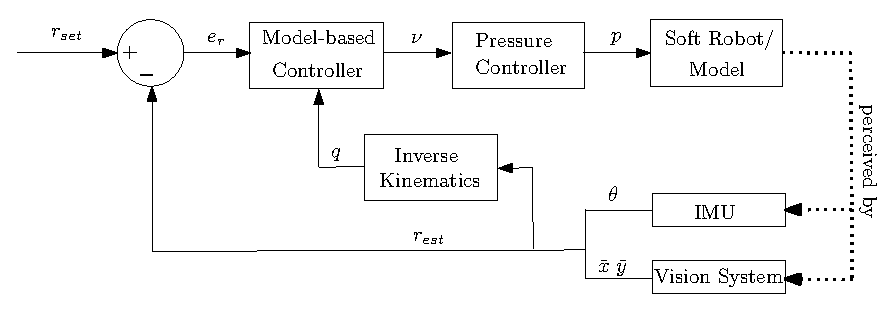
\includegraphics[width = \textwidth]{Figures/Chapter3/controlschemeActual.eps}
    \caption{Control lay-out of the model-based controller accompanied by a low-level pressure controller.}
    \label{fig4:controllayout}
\end{figure}




\section{Jacobian model based controller}


For controlling the soft robot, a model based controller is proposed based on the system's Jacobian matrix. As mentioned in Chapter \ref{chapter1} this method has readily been applied to the field of soft robotics. 


To control the soft robot a Jacobian based model based controller is proposed. Jacobian control is widely applied for position control of classic robots. However, this theory can also be applied to soft robots given that the Jacobian can be calculated. In this work, a Jacobian PI controller is implemented \cite{MOOSAVIAN20071226}. The latter work states that a computed torque controller can be approximated by a more straightforward control law involving the Jacobian transpose. This approximation holds if high enough control gains are used. The Jacobian controller that is to be implemented is given by,


\begin{equation}
    \nu_{set} = \begin{bmatrix}J_c(\sigma,t)\end{bmatrix}_1^\top \Big(K_p e_r + K_i \int_0^t e_r \hspace{2pt} ds \Big) \hspace{10pt} \text{with} \hspace{10pt} e_r = e_{set}-e_{est}, 
    \label{eq:tau}
\end{equation}

where the proportional-integrator structure can be directly observed. Due to the structure of the control architecture the controller does not 

In this controller, diagonal gain matrices $K_p$ and $K_i$ both in $\mathbb{R}^{2\times 2}$ contain proportional and integrator gains, respectively. 


The controller designed in this study includes jacobian information. Jacobian control is a widely applied type of model-based controller for positioning classic robots. As mentioned in Chapter \ref{chapter1}, Jacobian controllers only use model information on velocity and position level. Thus, system dynamics are not used in this control law

where $\nu_{set} \in \mathbb{R}^2$ is the control input vector with control input moment and force. The Jacobian is determined with equation \ref{eq2:J}. Furthermore, $K_p$ and $K_i \in \mathbb{R}^{2\times 2}$ are diagonal gain matrices. Here $K_p$ penalizes proportional to the error, $K_i$ contributes to the sum of the error over time. The error $e_r \in \mathbb{R}^2$ is defined as the difference between reference position and the actual position in the (x,y)-plane. Therefore not the entire Jacobian of dimension $3 \times 2$, but only the entries mapping modal coordinate velocity to linear velocity in x-y plane $J_c$, corresponding to the second and third row. As mentioned this Jacobian is space-time variant. Therefore, in the control law this Jacobian is calculated real-time based on the actual kinematic configuration of the actuator. Based on the simplified inverse kinematics, that belong two a first order approximation. The simplified inverse kinematics are detailed in Appendix \ref{app4}.

\section{Pressure control}


The actual system does not allow to induce forces and moments directly. Therefore this control input should be mapped to pressure. Using the inverse of the mapping found by finite element analysis in Chapter \ref{chap3} desired input forces and moments can be mapped to pressure. Based on the desired control input, a reference pressure can be formulated as,

\begin{equation}
    p_{set} = H^{-1}\nu,
\end{equation}


where $p_{set} \in \mathbb{R}^2$ is the reference pressure for each bellow. In order for this reference pressure to be reached a second controller is necessary. This low-level controller is used to set the input voltage that is supplied to the air pumps. A standard PI-controller is deemed good enough to track the reference pressure. Therefore the control law is can be described by,

\begin{equation}
    V_{set} = K_{pp}e_p + K_{ip} \int_0^t e_p \hspace{2pt} ds \hspace{10pt} \text{with} \hspace{10pt} e_p = p_{set} - p,
\end{equation}



where $V_{set}$ is the input voltage based on the pressure error $e_p$. The proportional action is based on diagonal gain matrix $K_{pp} \in \mathbb{R}^{2\times 2}$. The integral action is done by $K_{ip}\mathbb{R}^{2\times 2}$.


\section{Digital Filters}


%Above state space model and presented Jacobian controller is implemented in \MATLAB. The used settings gains are $K_p = \text{diag}([400,400])$  and $K_i = \text{diag}([150,150])$. Figure  shows a simulation for a set point $q_{set} = [0 0.3]^\top$, which is equivalent to a position of [0,0.084]$m$ in the xy-plane.




%It is clear that since only a elongation is desired the pressure in both bellows should become equal. Therefore control input $V_1 = V_2$, and is saturated to the maximum 12V. Once the setpoint is nearly reached the control input slowly drops to ... V. It can be seen that the pump dynamics are the major limiting factor in the achievable performance of the set-up. The dynamic model simulations shown in Appendix \ref{app4} showed that for a free oscillation the settling time is in the order of 0.1 seconds. For this setpoint the settling time is around ... seconds. Clearly the actuator damping does not play a large role setpoint regulation. . As one can see the controller  


%Using the same tuning parameters a curvature set-point as $q_{set} = [10,0.3]$ can be simulated. 


%\begin{figure}
%    \centering
%    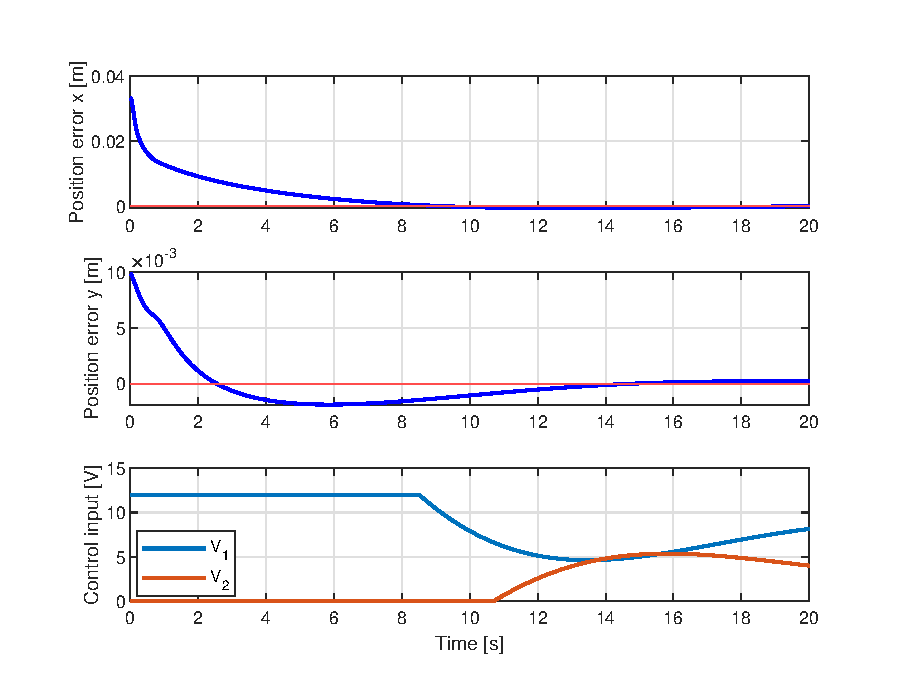
\includegraphics{Figures/Chapter4/k10e03.eps}
 %   \caption{Caption}
%    \label{fig:my_label}
%\end{figure}


























%The proposed Jacobian controller can be improved by adding additional model information. A major improving factor to the performance of the controller is adding stiffness compensation. Since the set-point is known, the necessary stiffness force and moment at that position are known. This compensation can directly be added to the control signal. The resulting controller then is,


%\begin{equation}
  %  \tau_{set} = \begin{bmatrix}J(\sigma,t)\end{bmatrix}^\top \Big(K_p e %+ K_i \int_0^t e \hspace{2pt} ds +  K_d \dot{e}\Big) + %\begin{bmatrix} K_\kappa(\kappa_{set}) & 0 \\ 0 & %K_\epsilon(\epsilon_{set}) \end{bmatrix} q_{set} , 
%    \label{eq:tauK}
%\end{equation}

%where additionally the stiffness is evaluated at modal coordinate setpoint $q_{set}$